\newcommand{\CLASSINPUTtoptextmargin}{0.76in}
\newcommand{\CLASSINPUTbottomtextmargin}{1.1in}
\documentclass[conference]{IEEEtran}
\usepackage{colortbl}
\usepackage{amsmath}
\IEEEoverridecommandlockouts
\usepackage{cite}
\usepackage{amsmath,amssymb,amsfonts}
\usepackage[ruled,vlined,linesnumbered]{algorithm2e}
\usepackage[compatible]{algpseudocode}
% \usepackage{algorithmic}
\usepackage{caption}
\usepackage{subcaption}
\usepackage{algcompatible}
\usepackage{graphicx}
\setlength{\columnsep}{0.26in}
\usepackage{textcomp}
\usepackage{xcolor}
\def\BibTeX{{\rm B\kern-.05em{\sc i\kern-.025em b}\kern-.08em
    T\kern-.1667em\lower.7ex\hbox{E}\kern-.125emX}}
\begin{document}

\title{MAPPO-Based Multi-UAV Trajectory Optimization for AoI Minimization with Obstacle and Energy Awareness\\
}

\author{
\IEEEauthorblockN{Shilpi Kumari, Dev Gupta, Gaurav Rawat, Ajay Pratap}
\IEEEauthorblockA{\textit{Department of CSE, Indian Institute of Technology (BHU), Varanasi} \\
% \textit{IIT BHU}\\
% Varanasi, India \\
Email: \{shilpikumari.rs.cse21, dev.gupta.cse22, gaurav.rawat.cse22, ajay.cse\}@iitbhu.ac.in}
}
\maketitle

\begin{abstract}
Future wireless networks stand to gain significantly from integrating Unmanned Aerial Vehicles (UAVs) for on-demand data collection, particularly in defense scenarios. While existing UAV systems emphasize energy conservation, they often overlook data freshness, a critical factor in military missions across difficult terrains. This work presents a novel solution that jointly considers Age of Information (AoI) and energy efficiency in Multi-UAV assisted IoT networks tailored for such environments. By employing clustering and Deep Reinforcement Learning (DRL) for UAV position optimization, we effectively reduce both average AoI and energy usage. Our Multi-Agent Proximal Policy Optimization UAV Trajectory Planning (MAPPO-UTP) framework leverages Deep Neural Networks (DNNs) for informed and adaptive trajectory decisions.


\end{abstract}

\begin{IEEEkeywords}
UAV, Multi-Agent, IoT, AoI, Defense, Clustering, DRL.
\end{IEEEkeywords}

\section{Introduction}
% Unmanned Aerial Vehicles (UAVs) have emerged as pivotal assets in modern wireless networks, especially in mission-critical applications like defense surveillance and disaster management. In such scenarios, rapid and efficient data collection from widespread IoT devices is essential, not only to ensure real-time responsiveness but also to maintain the freshness of information. %~\cite{ lyu2022global,gong2023resilient}.
% These devices track parameters and facilitate real-time management in military operational zones, where the freshness of data is paramount for informed decision-making, crucial not only for civilian applications but also for national defense. Integrated into defense systems, IoTDs provide essential surveillance and reconnaissance data, enabling rapid responses to evolving threats and ensuring national security.

% However, the system's effectiveness can be compromised by outdated information, particularly in defense operations in rugged terrains. To address this challenge, we employ the Age of Information (AoI) metric, which assesses data freshness by measuring the time elapsed since the last status update~\cite{kosta2017age}. Yet, complexities emerge due to the geographical gap between Base Stations (BS), i.e., military centers, and IoTDs, amplified by challenging environmental conditions, such as remote hilly regions~\cite{liu2022aoi}. In defense scenarios, where real-time data is imperative for decision-making, delays in data collection could have severe consequences. Unmanned Aerial Vehicles (UAVs) offer a solution to mitigate this issue. Their versatility and mobility make them ideal for collecting IoTDs data. UAVs can serve as aerial base stations, enabling high-speed data transmission near IoTDs through Line-of-Sight (LoS) links.

Unmanned Aerial Vehicles (UAVs) are transforming the landscape of wireless communication, particularly in defense and mission-critical applications where timely data acquisition is essential. In such settings, Internet of Things Devices (IoTDs) are deployed to monitor and collect critical environmental and operational data. However, the vast deployment of these devices and their location in hostile or inaccessible terrains present challenges for timely data retrieval and task execution. Ensuring that the collected information remains fresh and actionable is vital for mission success. To this end, data freshness—quantified through the Age of Information (AoI)—becomes a crucial performance metric. In rugged military terrains, the distance between IoTDs and central Base Stations (BS) often results in significant communication delays, potentially compromising situational awareness and response effectiveness.Delayed or outdated data can severely hinder operational efficiency and responsiveness, especially in high-stakes defense missions requiring continuous situational awareness. Traditional ground-based networks often fall short in providing the needed coverage and adaptability in such environments.

To overcome these limitations, we propose a model that leverages UAVs not only as mobile relays but also as intelligent agents capable of adaptive trajectory planning and task offloading.UAVs have gained prominence as agile, mobile platforms capable of bridging the communication gap between IoTDs and central processing stations. Their ability to establish reliable Line-of-Sight (LoS) communication links and access otherwise unreachable areas offers a practical solution for data collection in harsh conditions. However, effective utilization of UAVs in such roles necessitates intelligent coordination, energy-aware planning, and data freshness optimization. Motivated by these needs, this work focuses on enhancing the performance and reliability of UAV-assisted IoT networks by exploring advanced task offloading and path planning strategies.

\section{Related Works}
% Numerous studies have concentrated on optimizing data collection ratios and reducing the AoI~\cite{liu2022aoi,baek2019energy}. Traditional methods like convex optimization theory, genetic algorithms, Dynamic Programming (DP), and others have been widely used to achieve global solutions in communication networks~\cite{liu2022aoi,baek2019energy}. However, these approaches often rely on precise optimization models and global information, which are impractical in real-world military operations in hilly areas.
Numerous works have aimed to enhance data collection efficiency and minimize the Age of Information (AoI)\cite{liu2022aoi,baek2019energy}. Conventional techniques such as convex optimization, genetic algorithms, and Dynamic Programming (DP) have been extensively employed to find optimal solutions within communication networks\cite{liu2022aoi,baek2019energy}. Nevertheless, these methods typically depend on accurate modeling and complete global knowledge, which can be challenging to obtain in practical military deployments, especially in rugged and mountainous terrains.

In addition to multi-UAV coordination strategies, several works have focused on task offloading and path planning using a single UAV. These models typically assume a single aerial agent responsible for collecting data from all IoTDs and offloading it to the base station~\cite{SingleAgentPPO}. While these systems simplify control and deployment, they often suffer from scalability issues and increased latency, particularly in large-scale or geographically complex environments. Despite achieving reasonable performance in smaller or less dynamic scenarios, single-UAV systems face limitations in meeting strict AoI and energy efficiency requirements in mission-critical settings, such as defense operations in hilly terrain. As a result, there is a growing interest in exploring multi-UAV frameworks to enhance robustness, reduce latency, and better adapt to dynamic environments.A comparative analysis of closely related works in the literature, as shown in Table \ref{RelWork}. 

% Actor-Critic is a reinforcement learning framework that combines two components: the actor, which decides the actions, and the critic, which evaluates how good those actions are based on a value function. This structure enables more stable learning compared to pure policy-based or value-based methods. However, in complex multi-UAV networks, traditional Actor-Critic methods often struggle due to the non-stationary nature of multi-agent environments.
% Multi-Agent Proximal Policy Optimization (MAPPO) allows for more stable and sample-efficient learning. MAPPO better manages coordination, credit assignment, and policy optimization among UAVs, making it more effective than standard Actor-Critic methods in dynamic multi-agent tasks like collaborative surveillance, area coverage, and rescue operations.


% In this paper, we formulate the utility maximization problem via covering clusters of IoTDs in hilly areas. UAVs are energy-constrained, and so their routes should be carefully planned, taking into account the overall maximized utility while avoiding various hilly obstacles along the way. This problem is very challenging, and therefore, we present a sub-optimal solution based on Deep Reinforcement Learning (DRL). In a nutshell, the main contributions of this work can be summarized as follows:
% \begin{itemize}
%     \item Formulate a novel optimization problem, aiming to maximize the utility of UAV.
%     \item Propose a sub-optimal DRL-based solution.  
%     \item Extensive performance assessment demonstrates the effectiveness of the proposed algorithm. 
% \end{itemize}
This paper focuses on the challenge of utility maximization for data collection in clustered IoT networks deployed across hilly terrains. Given the limited energy capacities of UAVs, it becomes crucial to design their flight paths in a way that maximizes overall utility while effectively navigating around natural obstacles. The complexity of this scenario makes exact optimization intractable; hence, we propose a sub-optimal yet efficient solution based on Deep Reinforcement Learning (DRL). Unlike traditional single-agent approaches, our model leverages a MAPPO framework that enables multiple UAVs to collaboratively coordinate their routes and tasks. We summarize the core contributions of this paper as follows:
\begin{itemize}
    \item A novel formulation of the UAV utility maximization problem in challenging terrain environments.
    \item A multi-agent DRL-based framework for scalable and adaptive path and task allocation.
    \item Comprehensive simulation results validating the superior performance and practicality of our proposed method.
\end{itemize}


% \section{Related Works}\label{table1}
% This section provides a comparative analysis of closely related
% works in the literature, as shown in Table \ref{RelWork}.


% \begin{table}
% \center
% 		\caption{Summary of related works}\label{RelWork}
% 		\begin{tabular}{|c|c|c|c|c|c|} 
% 		\hline 
% 			\textbf{Works} & \textbf{AoI} & \textbf{IoTD Clustering} & \textbf{Energy}  & \textbf{Collision detection} & \textbf{Multi-Agent}\\
%             \hline
%             \cite{sun2021aoi}\cite{yi2020deep} &  $\checkmark$ &$\times$ & $\checkmark$  & $\times$ & $\times$ \\
%             \hline
%             \cite{xu2020big} &  $\checkmark$ &$\times$ & $\checkmark$  & $\times$ & $\checkmark$ \\
% 			\hline
%    %          \cite{aoimin}&  $\checkmark$ &$\checkmark$& $\checkmark$ & $\checkmark$ \\
% 			% \hline
%             % \cite{xu2020big} &  $\checkmark$ & $\times$ & $\checkmark$ & $\times$ \\
%             % \hline
%             \cite{zhan2019completion}&  $\times$ &$\checkmark$& $\checkmark$ & $\times$ &$\checkmark$\\
%             \hline
%             \cite{liu2022drl} &  $\times$ &$\checkmark$& $\checkmark$ & $\times$  & $\times$ \\
%             \hline
%             \cite{wan2024deep}&  $\times$ &$\times$& $\times$ & $\times$ &$\checkmark$\\
%             \hline
%             \cite{hu2022obstacle} &  $\times$ &$\times$& $\times$ & $\times$ & $\times$\\
%             \hline
%             % \cite{yi2020deep}&  $\checkmark$ &$\times$& $\checkmark$ & $\times$ \\
%             % \hline
%             \cite{zhou2024optimization}&  $\checkmark$ &$\checkmark$& $\checkmark$ & $\times$ & $\times$\\
%             \hline
%             \cite{SingleAgentPPO} &  $\checkmark$ &$\checkmark$& $\checkmark$ & $\checkmark$ & $\times$\\
%             \hline
%             Ours & $\checkmark$ &$\checkmark$& $\checkmark$ & $\checkmark$ & $\checkmark$\\
%             \hline
%     %         \cite{liu2022drl}&  $\times$ &$\checkmark$& $\checkmark$ & $\times$ \\
% 		  % \hline
%             % \cite{hu2022obstacle}&  $\times$ &$\times$& $\times$ & $\times$\\
% 		% \hline
% 		\end{tabular}
% \end{table}

\begin{table}[h]
\center
\caption{Summary of related works}\label{RelWork}
\resizebox{0.5\textwidth}{!}{%
\begin{tabular}{|c|c|c|c|c|c|} 
	\hline 
	\textbf{Works} & \textbf{AoI} & \textbf{IoTD Clustering} & \textbf{Energy}  & \textbf{Collision detection} & \textbf{Multi-Agent}\\
	\hline
	\cite{sun2021aoi}\cite{yi2020deep} &  $\checkmark$ &$\times$ & $\checkmark$  & $\times$ & $\times$ \\
	\hline
	\cite{xu2020big} &  $\checkmark$ &$\times$ & $\checkmark$  & $\times$ & $\checkmark$ \\
	\hline
	\cite{zhan2019completion}&  $\times$ &$\checkmark$& $\checkmark$ & $\times$ &$\checkmark$\\
	\hline
	\cite{liu2022drl} &  $\times$ &$\checkmark$& $\checkmark$ & $\times$  & $\times$ \\
	\hline
	\cite{wan2024deep}&  $\times$ &$\times$& $\times$ & $\times$ &$\checkmark$\\
	\hline
	\cite{hu2022obstacle} &  $\times$ &$\times$& $\times$ & $\times$ & $\times$\\
	\hline
	\cite{zhou2024optimization}&  $\checkmark$ &$\checkmark$& $\checkmark$ & $\times$ & $\times$\\
	\hline
	\cite{SingleAgentPPO} &  $\checkmark$ &$\checkmark$& $\checkmark$ & $\checkmark$ & $\times$\\
	\hline
	Ours & $\checkmark$ &$\checkmark$& $\checkmark$ & $\checkmark$ & $\checkmark$\\
	\hline
\end{tabular}%
}
\end{table}


The remainder of the paper is structured as follows: Section III presents the system model while Section IV presents the problem formulation and provides a proof of its NP-Hardness. Section V proposes a solution. Section VI provides a performance evaluation to validate the efficacy of the proposed system. Finally, Section VII presents conclusions and future research directions.

\section{System Model}\label{sec:System Model} 

We examine a UAV-assisted IoT network as illustrated in (Fig \ref{fig}), in which IoTDs need to upload their data to BS, for surveillance and security purposes in the hilly border area. Because IoTDs are energy-constrained and lack dedicated bandwidth, they cannot directly send data to the BS. A UAV 
$u$ is thus dispatched to act as a mobile intermediary, collecting and uploading their data to the BS..Let
$\mathcal{N} = \{1, \ldots , n , \ldots , N\}$ be the IoTDs set, with $I_n(t)$ denoting the data size of IoTD $n \in \mathcal{N}$ at time $t$. To facilitate the data collection of UAV $u$, all IoTDs are divided into $M$ clusters, where $M < N$. Let $\mathcal{M} = \{1,\ldots, m , \ldots, M\}$ be the collection of clusters. Each cluster $m \in \mathcal{M}$ consists of one Cluster Head (CH) denoted as $c_m$, which collects data from each IoTD in its cluster and transfers it to UAV $u$.

% $\mathcal{N} = \{1, \ldots , n , \ldots , N\}$ is the IoTDs set.
% $\mathcal{M} = \{1,\ldots, m , \ldots, M\}$ is the set of clusters.

\begin{figure}[tbh!]
\centerline{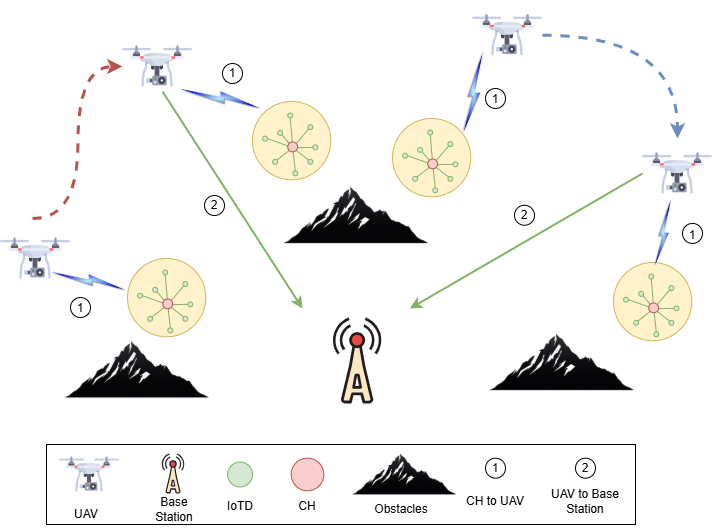
\includegraphics[width=\columnwidth]{SystemModel.png}}
\caption{System architecture.}
\label{fig}
\end{figure}
We introduce a binary-variable $X_{n,m}(t)$ to check the association of IoTD $n$ with cluster $m$ at time $t$ as:
\begin{equation}\label{binary-v} 
    X_{n,m}(t) = 
    \begin{cases}
        1, & \mbox{if IoTD } n \mbox{ belongs to cluster } m,\\ 
        0, & \mbox{otherwise}.
    \end{cases}
\end{equation}
We have assumed the IoTDs to be stationary in this paper so $X_{n,m}(t)$ will not change with time(is not a function of time) but in future it can be used to accomodate dynamic clustering if the IoTDs are not stationary.

Let $\ell_u(t) = [x_u(t),y_u(t),h_u(t)]$, $\ell_n(t)=[x_n(t),y_n(t),0]$, and $\ell_m(t)=[x_m(t),y_m(t),0]$ represent the 3-D coordinates of UAV $u$, IoTD $n \in \mathcal{N}$, and CH $c_m \in \mathcal{M}$, respectively.In our work we have assumed $h_u(t)$ to be constant, i.e., we have assumed that the UAV flies at a constant height. The UAV hovers in the air during data collection to optimize data transmission. We introduce a variable $Y_{u,m}(t)$ to indicate whether UAV $u$ is within the communication range of CH $c_m$ at time $t$ as follows:
\begin{equation}\label{u-range}
    Y_{u,m}(t) = 
    \begin{cases}
        1, & \mbox{provided UAV } u \mbox{ is within coverage area of CH } c_m,\\ 
        0, & \mbox{otherwise}.
    \end{cases}
\end{equation}
\subsection{IoTDs to CH transmission model}
When UAV $u$ gathers data directly from each IoTD, it must fly over individual IoTD locations, operating at peak power to maximize coverage of IoTDs within a defense monitoring zone. Simultaneously, IoTDs constantly search for the UAV to transmit data, causing high energy usage for both UAV and IoTDs. To reduce this, IoTDs are organized into clusters, each managed by a CH.
Hence, the data collection latency for CH $c_m$ from IoTDs in its assigned cluster is given by:
\begin{equation}
    T^{up}_m(t) = \max_{n\in\mathcal{N}}\left \{ X_{m,n}(t) \frac{I_n(t)}{R_{m,n}(t)} \right \}
\end{equation}
where $R_{m,n}(t)$ is the data rate between IoTD $n$ and CH $c_m$.
Similarly, the energy consumption between IoTD $n$ and CH $c_m$ can be defined as:
\begin{equation}
    E_{m,n}^{up}(t) = (P_n + P_m^{r})\left ( X_{m,n}(t) \frac{I_n(t)}{R_{m,n}(t)} \right )
\end{equation}

where $P_n$ is the transmitting power of IoTD $n$, and $P_m^{r}$ is the receiving power of CH $c_m$.

\subsection{CH to UAV transmission model}
Each cluster head (CH) $c_m$ continuously listens for the presence of UAV $u$. Once the UAV is detected within range, the CH initiates data transmission. The latency associated with this transmission from CH $c_m$ to UAV $u$ at time frame $t$ is given by:
\begin{equation}
    T_{m,u}^{up}(t) = \frac{\sum_{n=1}^{N} I_n X_{n,m}(t) Y_{u,m}(t)}{R_{m,u}(t)}
\end{equation}
where $R_{m,u}(t)$ denotes the data rate between CH $c_m$ and UAV $u$. Correspondingly, the energy consumed by CH $c_m$ during the transmission process can be expressed as:
\begin{equation}
    E_{m,u}^{up}(t) = P_m T_{m,u}^{up}(t)
\end{equation}
where $P_m$ represents the transmission power of CH $c_m$.

\begin{figure*}[htbp]
    \centering
`    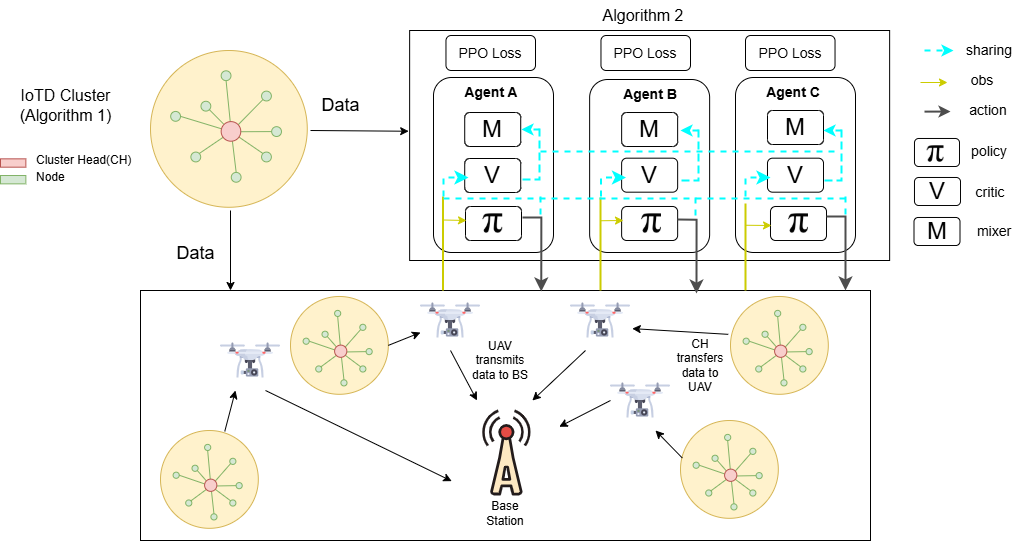
\includegraphics[width=\textwidth]{mappo.png}
    \caption{Multi-Agent Proximal Policy Optimization}
    \label{fig:mappo}
\end{figure*}

\begin{figure*}[htbp]
    \centering
`    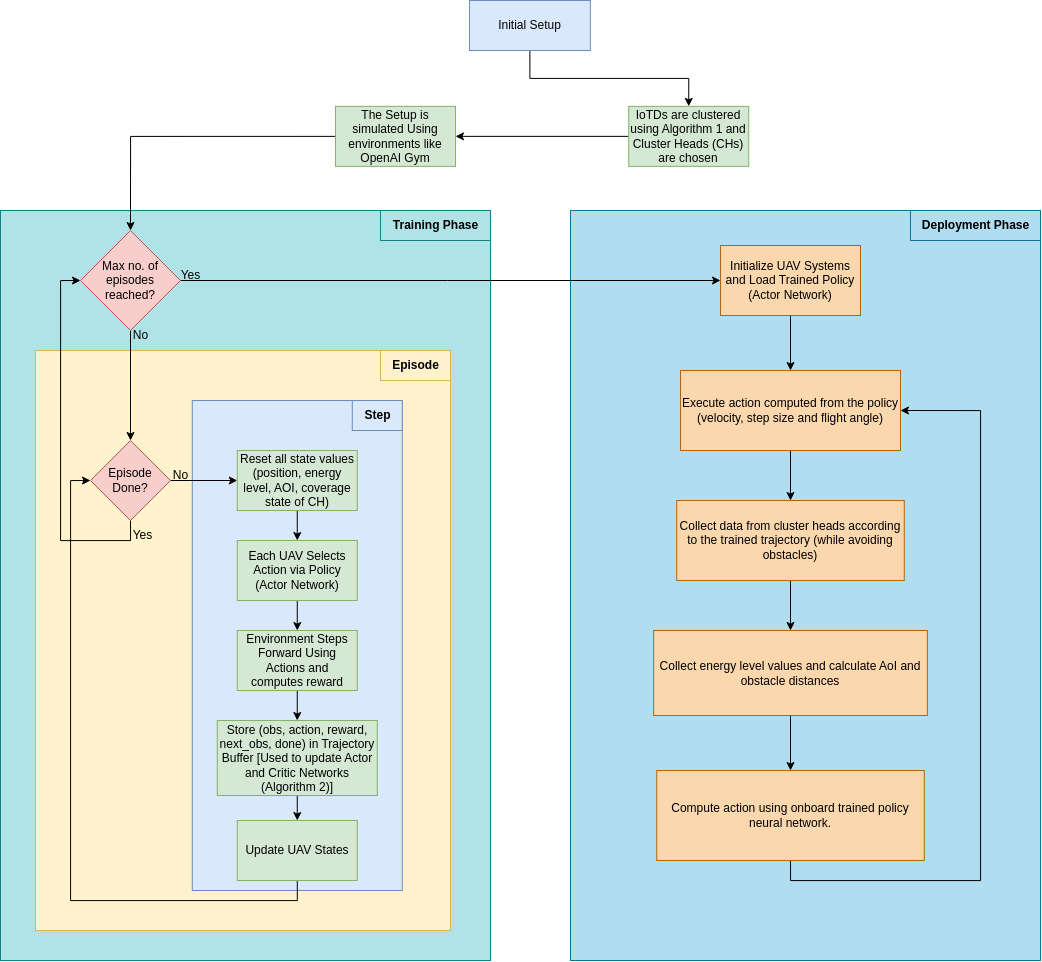
\includegraphics[width=\textwidth]{flowchart.png}
    \caption{Execution Flowchart}
    \label{fig:flowchart}
\end{figure*}

\subsection{UAV traversal and transmission model}
The UAV flies over each CH to gather data. We assume the presence of $O$ fixed obstacles such as hills and trees within the area. Let $\mathcal{O} = {1, 2, \ldots, o, \ldots, O}$ represent the set of these obstacles, where each obstacle has 3D coordinates denoted by $\ell_o = [x_o, y_o, h_o]$. To prevent collisions, the UAV maintains a minimum safe distance $d_s$ from all obstacles. The potential collision state between UAV $u$ and any obstacle $o$ can be represented by:
\begin{equation}\label{binary-v3} 
    C_{u,o}(t) = 
    \begin{cases}
        1, & \mbox{if $d_{u,o}(t)$ is less than $d_s$} ,\\ 
        0, & \mbox{otherwise}
    \end{cases}
\end{equation}
The number of collisions at time $t$ for a UAV $u$ can be given by :
\begin{equation}
    % Z(t) = \sum_{o=1}^OC_{u,o}(t)
    Z_u(t) = \sum_{o=1}^O C_{u,o}(t)  
\end{equation}
The traversal time of UAV $u$ to reach over CH $c_m$ for data collection can be calculated as:
\begin{equation}
    T_{m,u}^{trav}(t) = \frac{d_{m,u}}{v_u(t)} 
\end{equation}
Here $d_{m,u}$ denotes the distance travelled by the UAV to reach CH $m$ at time $t$ and $v_u(t)$ represents the UAV's velocity at that time.The traversal energy of UAV $u$ to reach over CH $c_m$ for data collection can be given by:
\begin{equation}
    E_{m,u}^{trav}(t) =  T_{m,u}^{trav}(t) P_{u}^{trav}
\end{equation}
%define Ptravel here
where $P_{u}^{trav}$ represents the power consumed by the UAV during traversal.
The UAV must remain stationary above each CH $c_m$ until it has received the complete data transmission. Therefore, the energy consumed by UAV $u$ due to hovering can be expressed as:
\begin{equation}
    E_{m,u}^{hov}(t) =  T_{m,u}^{up}(t) P_{u}^{h}
\end{equation}
Here, $P_{u}^h$ denotes the hovering power of UAV $u$. It is assumed that the data gathered from each CH is offloaded to the BS before the UAV reaches its next hovering position. The energy consumed by UAV $u$ to transmit the data from CH $c_m$ can be computed as:
\begin{equation}
    E_{u,BS}^{up}(t) = \frac{I_u(t)}{R_{u,BS}(t)} P_u^{trans}
\end{equation}
Here, $P_u^{trans}$ denotes the transmission power of the UAV, and $R_{u,BS}(t)$ represents the rate of data exchange between the UAV and the BS. The term $I_u(t)$ refers to the amount of data stored on the UAV after receiving it from CH $c_m$, and is given by:
\begin{equation}
    I_u(t) = \sum_{n=1}^{N}I_n(t)X_{m,n}(t)Y_{u,m}(t)
\end{equation}
\subsection{AoI}
We define \textit{AoI} as a crucial performance measure that captures the time duration since the latest received data was initially generated in the defense surveillance region. The \textit{AoI} for cluster head $m$ at the $t^{th}$ time frame is evaluated as:
\begin{equation}\label{binary-v2} 
    A_m(t) = 
    \begin{cases}
       T_{m,u}^{trav}(t) + T_{m,u}^{up}(t) & \mbox{if }Y_{u,m}(t)=1 \\ 
       & \\
        A_m(t-1) +  T_{m',u}^{trav}(t)  & \mbox{if } m' \neq m\\
        + T_{m',u}^{up}(t)&Y_{u,m'}(t) = 1.
    \end{cases}
\end{equation}
The average AoI of all CHs at $t^{th}$ time frame is given as:
\begin{equation}
    A(t) = \frac{1}{M} \sum_{m=1}^M A_m(t)
\end{equation}
\section{Problem Formulation and NP Hardness Proof}
This study focuses on reducing the weighted sum of AoI and energy usage by both UAVs and IoTDs, while ensuring collision avoidance in the mountainous military terrain. Consequently, the utility function is formulated as:
% \begin{equation}
% \begin{split}
%     U &= \frac{1}{\mathcal{T}} \sum_{t=1}^\mathcal{T} ( w_1E\left[-A(t)\right] +w_2E\left[-\mathcal{E}_{u}(t)\right] \\ 
%     & + w_3E\left[-\mathcal{E}_{IoTD}(t)\right] + w_4E\left[-Z(t)\right] )
% \end{split}
% \end{equation}

% \begin{equation}
% \begin{split}
%     U &= \frac{1}{\mathcal{T}} \sum_{t=1}^\mathcal{T} \sum_{u=1}^\upsilon \left( w_1 E\left[-A_u(t)\right] + w_2 E\left[-E_u(t)\right] \right. \\
%     &\quad \left. + w_3 E\left[-E_{IoTD,u}(t)\right] + w_4 E\left[-Z_u(t)\right] \right)
% \end{split}
% \end{equation}

\begin{align}
U &= \frac{1}{\mathcal{T}} \sum_{t=1}^\mathcal{T} \bigg[ \sum_{u=1}^\upsilon \Big( w_1 E[-A_u(t)] + w_2 E[-E_u(t)] \notag \\
&\quad + w_4 E[-Z_u(t)] \Big) + w_3 E[-E_{IoTD}(t)] \bigg]
\end{align}

where $\mathcal{T}$ is the number of time frames. $w_1$, $w_2$, $w_3$, and $w_4$ are weight factors for average AoI, UAV energy, IoTD energy, and collision penalty, respectively, and $\upsilon$ is the total number of UAVs.
$E_u(t)$ is given by:
\begin{equation}
    E_{u}(t) = \sum_{m=1}^{M}\left (  E_{m,u}^{trav}(t) + E_{m,u}^{hov}(t) +  E_{u,BS}^{up}(t)\right )Y_{u,m}(t)
\end{equation}

Similary, $E_{IoTD}(t)$ can be given as :

\begin{equation}
\begin{split}
    E_{IoTD}(t) & = \sum_{m=1}^{M}\sum_{n=1}^{N}E_{m,n}^{up}(t)X_{m,n}(t) \\
    &+   \sum_{m=1}^{M} E_{m,u}^{up}(t)Y_{u,m}(t)
    \end{split}
\end{equation}

\subsection{Problem Formulation}
\noindent Our problem function is formulated as :
\begin{equation}\label{eq:opt-function}
    \textbf{P} :\quad \text{max} \quad U 
\end{equation}
% \begingroup
% \allowdisplaybreaks
% \begin{align}    
%      & \sum_{t=1}^{\mathcal{T}} \mathcal{E}_{u}(t) \leq \mathcal{E}_u^{max} \tag{\ref{eq:opt-function}a}\label{eq:c1} ,\\
%      & v_u(t) \leq v_u^{max},  \forall t \in \mathcal{T} \tag{\ref{eq:opt-function}b} \label{eq:c2} ,\\
%      % & h_{min} \leq h_u(t) \leq h_{max},  \forall t \in \mathcal{T} \tag{\ref{eq:opt-function}c} \label{eq:c3} ,\\
%     & x_{min} \leq x_u(t) \leq x_{max} , y_{min} \leq y_u(t) \leq y_{max}
%     \tag{\ref{eq:opt-function}c}\label{eq:c4} ,\\
%     &  d_{u,o}(t) \geq d, \forall o \in \mathcal{O}
%     \tag{\ref{eq:opt-function}d}\label{eq:c5}\\
%     &  0 \leq w_1 + w_2 + w_3 + w_4 \leq 1	
%     \tag{\ref{eq:opt-function}e}\label{eq:c6}
% \end{align}
% \endgroup

\begingroup
\allowdisplaybreaks
\begin{align}    
     & \sum_{t=1}^{\mathcal{T}} E_{u}(t) \leq E_u^{max} \tag{\ref{eq:opt-function}a}\label{eq:c1} ,\\
     & v_u(t) \leq v_u^{max},  \forall t \in \mathcal{T} \tag{\ref{eq:opt-function}b} \label{eq:c2} ,\\
     % & h_{min} \leq h_u(t) \leq h_{max},  \forall t \in \mathcal{T} \tag{\ref{eq:opt-function}c} \label{eq:c3} ,\\
    & y_{min} \leq y_u(t) \leq y_{max} , x_{min} \leq x_u(t) \leq x_{max}
    \tag{\ref{eq:opt-function}c}\label{eq:c4} ,\\
    &  d_{u,o}(t) \geq d_s, \forall o \in \mathcal{O}
    \tag{\ref{eq:opt-function}d}\label{eq:c5}\\
    &  0 \leq w_1 + w_2 + w_3 + w_4 \leq 1	
    \tag{\ref{eq:opt-function}e}\label{eq:c6} ,\\
    & C_{max}^n(t) = h_u(t)\tan(\phi_n).
    \tag{\ref{eq:opt-function}f}\label{eq:c7} ,\\
    & \|p_n(t) - p_j(t)\| \geq [C_{max}^n(t) + C_{max}^j(t)] , \forall n, j, n \neq j.
    \tag{\ref{eq:opt-function}g}\label{eq:c8} ,\\
    & \|\ell_n(t) - \ell_j(t)\| \geq D_{min}, \forall n, j, n \neq j.
    \tag{\ref{eq:opt-function}h}\label{eq:c9}
\end{align}
\endgroup



Equation~\eqref{eq:c1} guarantees that the total energy consumed by UAV $u$ remains within its maximum energy capacity $E_u^{max}$. Equation~\eqref{eq:c2} imposes a constraint that the velocity of the UAV at any time $t$ must remain below the maximum permissible velocity $v_u^{max}$.Equation~\eqref{eq:c4} confines the UAV's location to remain within the specified boundaries of the service area, given by $x_{min}$, $x_{max}$, $y_{min}$, and $y_{max}$. According to Equation~\eqref{eq:c5}, the UAV must maintain a safe minimum distance $d_s$ from any obstacle $o \in \mathcal{O}$. Equation~\eqref{eq:c6} ensures that the combined weight factors remain within the [0, 1] range. Equation~\eqref{eq:c7} derives the maximum horizontal coverage radius $C_{max}^n(t)$ of UAV $u$ at time $t$, based on its altitude ($h_u$) and the maximum elevation angle $\phi_u$. In Equation~\eqref{eq:c8}, $v_u(t)$ represents the UAV’s 2D coordinates as $p_u(t) = [x_u(t), y_u(t)]^T$. This equation enforces the non-overlapping constraint to ensure that coverage areas of any two UAVs do not intersect. Lastly, Equation~\eqref{eq:c9} introduces the collision avoidance constraint, mandating that the separation between any two UAVs must be at least $D_{min}$ to prevent collisions.

\subsection{NP-Hardness Proof}
The UAV path planning problem for IoT data collection with energy and AoI minimization is NP-hard.

To prove that this problem is NP-hard, we demonstrate that the Traveling Salesman Problem (TSP), which is known to be NP-hard, can be reduced to this problem in polynomial time.

Consider a special case of the UAV path planning problem with the following parameters:
\begin{itemize}
    \item Set $\alpha = 1$ (weight for energy consumption)
    \item Set $\beta = 0$ (weight for AoI)
    \item Define energy consumption $E_u(p)$ as directly proportional to the Euclidean distance traveled along path $p$
    \item Require that the UAV must return to its starting position after visiting all IoT devices
\end{itemize}

Under these conditions, the problem reduces to:
\begin{equation}
    p^* = \arg\min_{p \in P} \{E_u(p)\} = \arg\min_{p \in P} \{d(p)\}
\end{equation}
where $d(p)$ represents the total Euclidean distance of path $p$.

This is precisely the definition of the Euclidean Traveling Salesman Problem: finding the shortest path that visits each point exactly once and returns to the starting point. Since TSP is NP-hard, and this problem contains TSP as a special case, the UAV path planning problem is at least as hard as TSP, making it NP-hard.

Moreover, the addition of AoI considerations ($\beta > 0$) introduces time-dependent costs and further increases the problem complexity, as it creates a multi-objective optimization problem with time-sensitive constraints. This makes the problem a variant of the TSP with time windows, which is known to be strongly NP-hard.

\subsection{Complexity Analysis}
The UAV path planning problem exhibits several characteristics that contribute to its computational complexity:

\begin{enumerate}
    \item \textbf{Combinatorial Explosion:} For $N$ IoT devices, there are $(N!)$ possible visitation sequences, making exhaustive search intractable for large instances.
    
    \item \textbf{Dynamic Costs:} The AoI increases with time, creating a time-dependent cost function where the cost of visiting a node depends on when it is visited.
    
    \item \textbf{Multi-objective Optimization:} The problem involves balancing two potentially conflicting objectives: minimizing energy consumption and minimizing AoI.
    
    \item \textbf{Spatial-Temporal Coupling:} Decisions about the spatial path directly impact the temporal aspects (AoI), creating complex interdependencies.
\end{enumerate}

% \subsection{Implications for Algorithm Design}
% Given the NP-hardness of the problem, exact algorithms are unlikely to scale efficiently for large instances. Instead, the following approaches may be more practical:

% \begin{itemize}
%     \item \textbf{Approximation Algorithms:} Algorithms that provide solutions within a provable factor of the optimal solution.
    
%     \item \textbf{Heuristic Methods:} Techniques such as genetic algorithms, simulated annealing, or ant colony optimization that can find good solutions in reasonable time.
    
%     \item \textbf{Problem Decomposition:} Breaking the problem into subproblems, such as clustering IoT devices and solving for optimal paths within clusters.
    
%     \item \textbf{Machine Learning Approaches:} Using reinforcement learning or other ML techniques to learn near-optimal policies for UAV routing.
% \end{itemize}


\begin{algorithm}
\SetKwInput{KwData}{Input}
\SetKwInput{KwResult}{Output}
\KwData{The positions of the $\mathcal{N}$ nodes ${p_{n_1}, \ldots, p_{n_N}}$ within the region, the cluster radius $R$, UAV flight altitude $h$, flight speed $v_u$, and additional system parameters.}
\KwOut{A reduced set $\mathcal{M}$ containing information of cluster heads and corresponding nodes.}
Initialization: Initialize related parameters\;
\For{i = 1 to N}{
$temp_{{C}_i} \gets \text{cluster formation results}$\;
$temp_{{CH}_i} \gets \text{group of cluster heads}$\;
$temp_{{C\_size}_i} \gets \text{cluster size}$\;
}
$M \gets \min\text{size}(CH)$ \;
$C \gets temp_C,$ \;
$CH \gets temp_{CH}$ \;
$C_size \gets temp_{C\_size}$ \;
Use the coordinates of the cluster head (CH) and data collector (DC) to solve subproblem 1, then optimize the UAV trajectory
V, and determine the optimal solution for subproblem 2.\;
\For{i = 1 to C do}{
\For{k = 1 to {C\_size(j)} do}{
Determine the optimal sequence for collecting data from member nodes within a cluster to solve subproblem 3 effectively. \;
}
}
\caption{Clustering Algorithm}
\label{cluster}
\end{algorithm}

% \begin{algorithm}
% \SetKwInput{KwData}{Input}
% \SetKwInput{KwResult}{Output}
% \KwData{Set of cluster heads $CH$, Number of clusters $n_u$}
% \KwResult{Set of collection regions $CR$}
% Initialization: Randomly select $k$ points from $CH$ as initial RIPs $RIPs$\;
% \Repeat{No significant change in cluster assignments}{
%     \For{each point $p \in CH$}{
%         $closest\_cluster \gets \argmin_{c_r \in RIP} d(p, c_r)$\;
%         Assign point $p$ to $closest\_cluster$\;
%     }
    
%     \For{each cluster $c \in C$}{
%         $new\_RIP \gets \text{Calculate mean of all points in cluster } c$\;
%         \If{$new\_RIP \neq current\_centroid$}{
%             Update cluster head $RIP_c$ to $new\_RIP$\;
%         }
%     }
    
%     $M \gets \text{Minimum cluster size}$\;
%     $n_u \gets \text{Number of UAVs}$\;
% }
% \For{each cluster $c \in C$}{
%     Determine optimal node visitation order within cluster\;
% }
% \caption{K-Means Clustering and Optimization Algorithm}
% \label{kmeans_clustering}
% \end{algorithm}




% \begin{algorithm}
% Initialize actor net and critic net parameters. \label{B1}\\
% % Initialize old actor net parameter\label{B2}\;
%         \For {each episode}{ \label{B3}
%             Reset the environment and initial state. Set $r=0$. \label{B4}\\
%             Execute k-means based clustering algorithm. \label{B5}\\
%             \For {each time stamp t}{ \label{B6}
%                Select action $a(t)$ from $s(t)$ based on policy. \label{B7}\\
%                Execute action $a(t)$ then obtain reward $r(t)$ and the next state $s(t+1)$. \label{B8}\\
%                Store $(s(t), a(t), r(t), s(t+1)$ into replay buffer. \label{B9}\\ 
%                Compute advantages based on current value function \label{B12}\;
%                Update the policy via Adam.\\
%                Fit the value function by taking $\tau$ steps of minibatch regression on TD-error.\\
%             }    
%         }
% \caption{Proximal Policy Optimization (PPO)}
% \label{PPO}
% \end{algorithm}



% \begin{algorithm*}
% \caption{Multi-Agent Proximal Policy Optimization (MAPPO)}
% \begin{algorithmic}[1]
% \REQUIRE Actor and critic network parameters $\theta$ and $\phi$.
% \FOR{each episode do}
%     \STATE Reset the environment and initialize the global state $s_0$. Set $r = 0$.
%     \FOR{each time step $t$ do}
%         \FOR{each agent $i$}
%             \STATE Select action $a_t^{(i)}$ from policy $\pi_\theta(a_t^{(i)} | o_t^{(i)})$, where $o_t^{(i)}$ is the local observation.
%             \STATE Execute joint action $\mathbf{a}_t = [a_t^{(1)}, \ldots, a_t^{(n)}]$, observe shared reward $r_t$, next global state $s_{t+1}$, and next local observations $\mathbf{o}_{t+1}$.
%         \ENDFOR
%         \STATE Store $(s_t, \mathbf{o}_t, \mathbf{a}_t, r_t, s_{t+1}, \mathbf{o}_{t+1})$ in the replay buffer.
%     \ENDFOR
%     \STATE Compute advantage estimates $A_t^{(i)}$ using Generalized Advantage Estimation (GAE).
%     \STATE Normalize advantages for stability.
% \ENDFOR

% \STATE \textbf{Update the policy and value networks:}
% \STATE \textbf{For each mini-batch of data:}
% \STATE Update the actor network parameters $\theta$ by maximizing the clipped PPO objective:
% \[
% L(\theta) = \mathbb{E}\left[\min(r_\theta A,\ \text{clip}(r_\theta, 1 - \epsilon, 1 + \epsilon)\,A)\right],
% \]
% where $r_\theta = \frac{\pi_\theta(a|o)}{\pi_{\text{old}}(a|o)}$.

% \STATE Update the critic network parameters $\phi$ by minimizing the clipped value loss:
% \[
% L(\phi) = \mathbb{E}\Bigl[\max\Bigl((V_\phi(s) - R)^2,\ \bigl(\text{clip}(V_\phi(s), V_{\phi_{\text{old}}}(s)-\epsilon,\ V_{\phi_{\text{old}}}(s)+\epsilon) - R\bigr)^2\Bigr)\Bigr],
% \]
% where $R$ is the normalized return.

% \STATE Use Adam optimizer for both updates.
% \STATE Repeat until convergence or maximum steps are reached.

% \end{algorithmic}
% \end{algorithm*}

\begin{algorithm}
\SetKwInput{KwData}{Input}
\SetKwInput{KwResult}{Output}
\KwData{Coordinates of IoT devices $\mathcal{N} = \{p_{n_1}, \ldots, p_{n_N}\}$, cluster heads $\mathcal{M} = \{p_{m_1}, \ldots, p_{m_K}\}$, UAVs $\mathcal{U} = \{p_{u_1}, \ldots, p_{u_U}\}$, obstacles $\mathcal{O}$ = $\{p_{o_1}, \ldots, p_{o_O}\}$, actor-critic network parameters $\theta$ and $\phi$}
\KwResult{Optimized policy networks $\pi_{\theta}$ for each UAV for visiting all cluster heads}

Initialize actor networks $\pi_{\theta}$ and critic networks $V_{\phi}$ for each UAV\;

\For{each episode}{
    Reset environment and set $\mathcal{V} \leftarrow \emptyset$ \tcp*[r]{Visited cluster heads}
    
    \While{$\mathcal{V} \neq \mathcal{M}$ \textbf{and} $t < \text{max\_steps}$}{
        \For{each UAV $u_i \in \mathcal{U}$}{
            Observe $o_t^{(i)}$ (includes nearby obstacles, unvisited cluster heads)\;
            Select action $a_t^{(i)} \sim \pi_{\theta}(a_t^{(i)} | o_t^{(i)})$ \tcp*[r]{Movement direction}
        }
        Execute joint action $\mathbf{a}_t$ and move UAVs accordingly\;
        Update $\mathcal{V}$ with newly visited cluster heads\;
        Compute reward $r_t$ based on visits, collisions, and energy consumption\;
        Store transition $(s_t, \mathbf{o}_t, \mathbf{a}_t, r_t, s_{t+1}, \mathbf{o}_{t+1})$\;
    }

    Compute advantage estimates $A_t^{(i)}$ using GAE for each UAV\;

    \For{$K$ epochs}{
        \For{each mini-batch from collected data}{
            Update $\theta$ by maximizing clipped PPO objective:\;
            \[
                L(\theta) = \mathbb{E}\left[\min\left(r_\theta A,\, \text{clip}(r_\theta, 1 - \epsilon, 1 + \epsilon)\cdot A\right)\right]
            \]
            Update $\phi$ by minimizing value loss\;
        }
    }
}
\caption{MAPPO for UAV Cluster Head Data Collection}
\label{mappo}
\end{algorithm}



\section{Proposed Solution}
We solve the formulated problem outlined in Eq. (\ref{eq:opt-function}) in three steps. 
\subsection{IoTD-CH clustering}
First, we use a k-means-based clustering algorithm to find CHs (Algorithm 1) to segregate IoTDs into clusters and assign cluster heads to each cluster(Fig. 3).
% \subsection{CR-RIP clustering}
% In the second phase, we divide all cluster heads into collection regions (CRs) and assign Region Identification Points (RIPs) such that the number of CRs formed is equal to the number of UAVs. Then, each CR is assigned a UAV which will be responsible for collecting data from said CR. The initial hovering point for the UAV will be the RIP of its assigned cluster.
\subsection{MAPPO}
Multi-Agent Proximal Policy Optimization (MAPPO) is a reinforcement learning algorithm designed for scenarios where multiple agents interact in a shared environment, each optimizing its own behavior while contributing to a common goal. MAPPO extends the single-agent PPO framework by incorporating centralized training with decentralized execution: during training, each agent’s local policy benefits from access to global state information (via a shared critic), while at execution time, each agent acts using only its local observations. This design makes MAPPO robust in partially observable and cooperative settings, and it supports continuous action spaces, making it highly suitable for real-world robotic control and multi-UAV trajectory optimization.

In the context of our paper, MAPPO provides an ideal framework due to the complex, dynamic, and decentralized nature of the environment. Here, multiple UAV agents must simultaneously optimize their trajectories to minimize the AoI while considering physical obstacles, energy constraints, and the networked structure of CHs that aggregate IoTD data. Each UAV, as a MAPPO agent, receives local observations (e.g., nearby CHs, its current AoI levels, distance to obstacles, remaining energy) and computes an action (trajectory update). During training, the centralized critic uses the global state (e.g., AoI across all CHs, energy status of all UAVs) to guide the learning of the local policies, ensuring coordinated and globally optimal behaviors.

MAPPO was chosen for our research because it efficiently handles the cooperative yet decentralized UAV coordination challenge, where each UAV must make local decisions that are still aligned with a global objective — minimizing network-wide AoI while avoiding collisions and conserving energy. Its policy-clipping and shared value function help ensure training stability and scalability across multiple agents, making it well-suited for real-time, large-scale UAV networks in smart IoT-based sensing systems.
\subsection{Identification of optimal collection trajectory using MAPPO}
In the third phase, we strategically use a Multi-Agent PPO-based policy \cite{schulman2017proximal} to find an optimal trajectory of the UAVs based on the locations of CHs
In this setup, the UAVs are independent agents that learn and determine their next hovering location based on current environmental conditions and obstacles on the way. MAPPO employs a stochastic policy, ensuring automatic exploration. It collects a mini-batch of experiences from interactions with the environment to update the policy. After updating, a new batch is collected with the updated policy, classifying PPO as an on-policy algorithm. Its optimization strategy, which limits the policy update step, often results in more stable training and prevents drastic changes, making it well-suited for training systems like UAVs.

\subsection{MDP Formulation}
We consider the above-defined system model as an environment. Considering that each UAV's action may influence the environmental state, total utility is determined by the current state of the environment and the action of the UAV. Hence, the utility maximization problem can be re-formulated as a multi-agent MDP $\left \langle S, a, R, \epsilon, \gamma  \right \rangle$ where $S$ is state set of agent $u$, $a$ is action space of agent $u$, $\epsilon$ denotes the state transition probability, $R$ is reward function of agent $u$, and $\gamma \in [0,1]$ represents discount factor. A detailed description is provided in the following subsections.
\begin{table}
        \caption{Simulation parameters}
        \begin{tabular}{|c|c|c|c|}
            \hline
            \textbf{Parameter} & \textbf{Value}& \textbf{Parameter} & \textbf{Value}\\
            \hline
           $v_u$ & 10 m/s & $E_{u}^{max}$ & 1000 J ~\cite{sun2021aoi}\\
            $P_n$ & 0.1 Watts~\cite{xu2021joint} & $I_n$ & 5-10 KB\\
            $P^{trav}$ & [10-35] J/sec~\cite{lim2021towards} & N & $100$ \\
            Max. steps & 50 & Batch size& 256\\
           $r_m$ & 500 & $p$ & 100\\
            \hline
        \end{tabular}
    \label{parameterTable}
\end{table}

% \begin{table}
%         \renewcommand{\arraystretch}{1.3}
%         \caption{Symbol description}
%         \label{tab:SybDes}
%         \begin{tabular}{ p{0.85cm}|p{7.045cm} }
        
%             \textbf{Symb.} & \textbf{Description}\\			
%             \hline
%          $\mathcal{N}$ & Set of IoTDs \\
%         \rowcolor{gray!20}
         
%         $\mathcal{M}$ & Set of cluster heads \\
%         $I_n(t)$ & Data size of IoTD at $t$\\
%         \rowcolor{gray!20}
        
%         $r_o$ & Average radius of obstacle \\
%         $\mathcal{O}$ & Coordinates of obstacles \\
%         \rowcolor{gray!20}
        
%         $P_t$ & The position of UAV in the $t^{\text{th}}$ time interval \\
%         $H$ & Height of UAV \\
%         \rowcolor{gray!20}
        
%         $G(T_{m,t}^{0})$ & The power gain of the channel between the $m^{\text{th}}$ IOTD and the UAV \\
%         $P_n$ & Transmitting power of the $n^{\text{th}}$ IoTD \\
%         \rowcolor{gray!20}
%         $B$ & Available channel bandwidth \\
%         $R_{P_t,m}$ & Data transmission rate \\
%         \rowcolor{gray!20}
%         $\sigma^{2}$ & Additive white Gaussian noise \\
%         $d_{m,u}$ & Length of the flight segment from the last UAV position to the current CH \\
%         \rowcolor{gray!20}
%         $R_{m,n}$ & Transmission rate between IoTD and CH \\
%         $\beta_0$ & Reference channel gain of distance \\
%         \rowcolor{gray!20}
        
%         $d_{a,b}$ & Distance between $a$ and $b$ \\
%         $A(\tau)$ & AoI at time $\tau$ \\
%         \rowcolor{gray!20}
        
%         $U_{tip}$ & Tip speed of the rotor blade \\
%         $v_0$ & Mean rotor induced velocity in the hovering status \\
%         \rowcolor{gray!20}
        
%         $d_0$ & Fuselage drag ratio \\
%         $s$ & Rotor solidity \\
%         \rowcolor{gray!20}
        
%         $\rho$ & Mean air density \\
%         $\delta$ & Rotor disc area \\
%         \rowcolor{gray!20}
        
%         $P_0$ & Blade profile \\
%         $P_i$ & Induced power in the hovering state \\
%         \rowcolor{gray!20}
        
%         $P_h$ & Hovering energy consumption \\
%         $r_{w}$ & Wake radius \\
%         \rowcolor{gray!20}
        
%         $P_{wake}$ & Power consumed by the wake sensor equipped on the CH as the wake sensor is always active \\
        
%         $d_s$ & Minimum safe distance from an obstacle \\
%         \rowcolor{gray!20}
        
%         $C_o^{\text{t}}$ & Collision state of the UAV with obstacle $o$\\
        
%         $OC_o^{\text{t}}$ & Number of collisions at time frame $t$ \\
%         \hline
%         \end{tabular}
% \end{table}


\begin{table}
    \renewcommand{\arraystretch}{1.3}
    \caption{Symbol description}
    \label{tab:SybDes}
    \begin{tabular}{ p{0.85cm}|p{7.045cm} }
    
        \textbf{Symb.} & \textbf{Description}\\			
        \hline
        $\mathcal{N}$ & Set of IoTDs \\
        \rowcolor{gray!20}
        $\mathcal{M}$ & Set of cluster heads \\
        $X_{n,m}(t)$ & Variable to check association of IoTD $n$ with cluster $m$ at time $t$ \\
        \rowcolor{gray!20}
        $Y_{u,m}(t)$ & Variable used to determine if UAV $u$ is within the communication range of cluster head $c_m$ at time $t$\\
        $I_n(t)$ & Data size of IoTD at $t$\\
        \rowcolor{gray!20}
        $r_o$ & Average radius of obstacle \\
        $\mathcal{O}$ & Coordinates of obstacles \\
        \rowcolor{gray!20}
        % $P_t$ & The position of UAV in the $t^{\text{th}}$ time interval \\
        $h_u$ & Height of UAV (assumed to be constant) \\
        $G(T_{m,t}^{0})$ & The power gain of the channel between the $m^{\text{th}}$ IOTD and the UAV \\
        \rowcolor{gray!20}
        $P_n$ & Transmitting power of the $n^{\text{th}}$ IoTD \\
        $P_{r}^{m}$ & Receiving power of CH $c_m$ \\
        \rowcolor{gray!20}
        $B$ & Available channel bandwidth \\
        $R_{P_t,m}$ & Data transmission rate \\
        \rowcolor{gray!20}
        $\sigma^{2}$ & Additive white Gaussian noise \\
        $d_{m,u}$ & Length of the flight segment from the last UAV position to the current CH \\
        \rowcolor{gray!20}
        $R_{m,n}$ & Transmission rate between IoTD and CH \\
        $E_{m,n}(t)$ & Energy consumption between IoTD $n$ and CH $c_m$ \\
        \rowcolor{gray!20}
        $\beta_0$ & Reference channel gain of distance \\
        $d_{a,b}$ & Distance between $a$ and $b$ \\
        \rowcolor{gray!20}
        $A(\tau)$ & AoI at time $\tau$ \\
        $R_{m,u}(t)$ & Data rate between CH $c_m$ and UAV $u$ \\
        % $U_{tip}$ & Tip speed of the rotor blade \\
        % \rowcolor{gray!20}
        % $v_0$ & Mean rotor induced velocity in the hovering status \\
        % $d_0$ & Fuselage drag ratio \\
        \rowcolor{gray!20}
        % $s$ & Rotor solidity \\
        % $\rho$ & Mean air density \\
        \rowcolor{gray!20}
        % $\delta$ & Rotor disc area \\
        \rowcolor{gray!20}
        $P_0$ & Blade profile \\
        % \rowcolor{gray!20}
        % $P_i$ & Induced power in the hovering state \\
        $P_{u}^{h}$ & Hovering Power of UAV $u$ \\
        \rowcolor{gray!20}
        $r_{w}$ & Wake radius \\
        $P_{wake}$ & Power consumed by the wake sensor equipped on the CH as the wake sensor is always active \\
        \rowcolor{gray!20}
        $d_s$ & Minimum safe distance from an obstacle \\
        $C_{u,o}^{\text{t}}$ & Collision state of the UAV $u$ with obstacle $o$\\
        \rowcolor{gray!20}
        % $OC_o^{\text{t}}$ & Number of collisions at time frame $t$ \\
        $Z_u(t)$ & Number of collisions at time $t$ for UAV $u$ \\
        $v_u(t)$ & Velocity of the UAV $u$ \\
        \rowcolor{gray!20}
        $I_u(t)$ & Amount of data stored on the UAV $u$ after receiving it from CH $c_m$ \\
        $p_{n_i}$ & Position of 'i'th IoTD\\
        \rowcolor{gray!20}
        $p_{m_i}$ & Position of 'i'th CH\\
        $p_{u_i}$ & Position of 'i'th UAV\\
        \rowcolor{gray!20}
        $p_{o_i}$ & Position of 'i'th Obstacle\\
        \hline
    \end{tabular}
\end{table}


\subsubsection{State Space}
The state of the environment encompasses various aspects, such as the position of the UAV, its energy levels, the average AoI of all CHs, and coverage status of the CHs. 
Mathematically, the state space can be represented as:
\begin{equation}
    s(t) = \{\ell_u(t), \mathcal{E}_u(t), A(t), \mathcal{C}\}
\end{equation}
where  $\mathcal{C} = \{C_1(t), \dots, C_m(t), \dots, C_M(t)\}$ denotes the coverage condition of all clusters. Binary variable $C_m(t) = 1$ means that CH $m$ has been served, and vice versa.
\subsubsection{Action Space}
The action space of the UAV is:
\begin{equation}
    a(t) = \{v_u(t), l_u(t), \theta_u(t)\}
\end{equation}
where $l_u(t)$ represents the flight distance, and $\theta_u(t)$ denotes the flight angle of the UAV. 
\begin{figure}[htbp]
\centerline{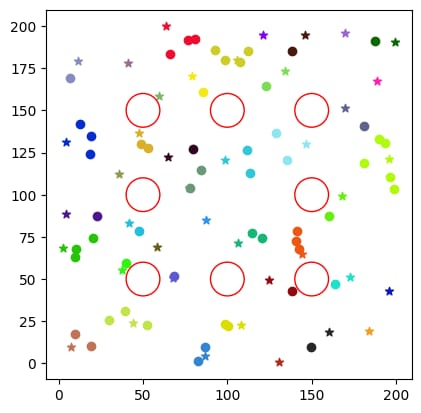
\includegraphics[width=1\columnwidth]{Clustering.png}}
\caption{Cluster heads.}
\label{p1}
\end{figure}
% \begin{figure}[htbp]
% \centerline{\includegraphics[width=1\columnwidth]{ch_rip_clustering.png}}
% \caption{Collection Regions}
% \label{p1}
% \end{figure}
\subsubsection{Reward}
The agent's reward is influenced by the average Age of Information (AoI) of the cluster heads, the energy consumption of IoTDs, and the energy usage of the UAV, and can be expressed as:
\begin{align}
    r(t) =\; & -w_1A(t) - w_2\sum_{u=1}^\upsilon E_{u}(t) - w_3E_{IoTDs}(t) \notag \\
             & - w_4\sum_{u=1}^\upsilon Z_{u}(t) + r_m - p
\end{align}

where $r_m$ is the positive reward that UAV $u$ receives for covering CH $m$, and $p$ is the penalty received by the UAV for each uncovered CH.


\section{Performance Study}
In this section, the training performance of the proposed algorithm is analyzed.
Simulation parameters used in the experiment are given in Table \ref{parameterTable}.

\begin{figure}[htbp]
\centerline{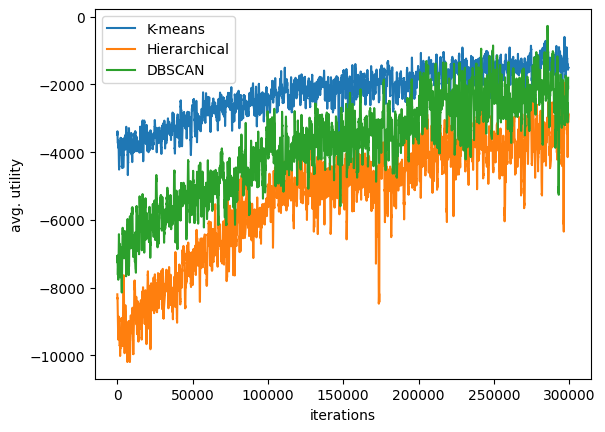
\includegraphics[trim=10 0 0 0, clip,width=1\columnwidth]{utilityVSclustering.png}}
\caption{Utility vs clustering scheme.}
\label{c1}
\end{figure}

\begin{figure}[htbp]
\centerline{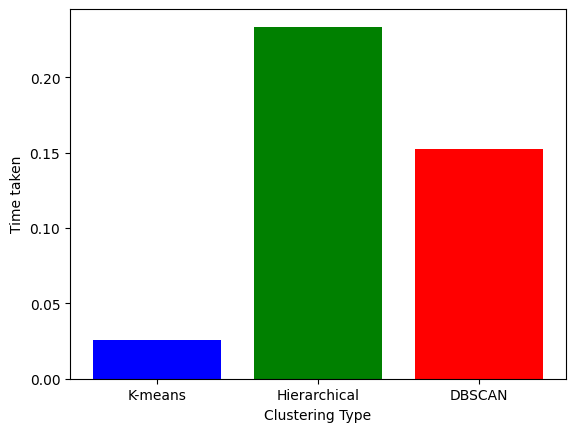
\includegraphics[trim=10 0 0 0, clip,width=1\columnwidth]{timeVSclustering.png}}
\caption{Time taken vs clustering scheme.}
\label{c2}
\end{figure}

\begin{figure}[htbp]
\centerline{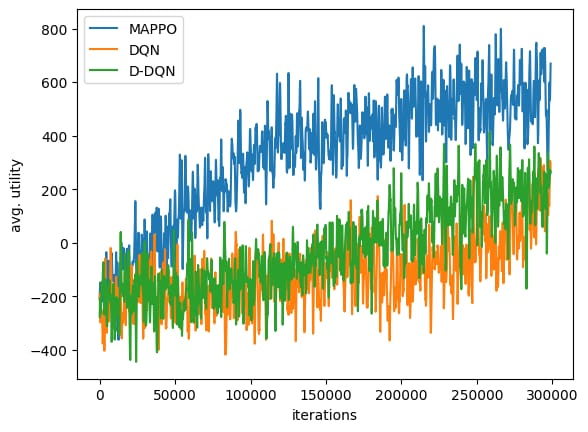
\includegraphics[trim=10 0 0 0, clip,width=1\columnwidth]{Utility_final.png}}
\caption{Avg. Utility vs iterations.}
\label{p2}
\end{figure}
% \begin{figure}[htbp]
% \centerline{\includegraphics[width=1\columnwidth]{Explo2.png}}
% \caption{Avg. steps vs episodes.}
% \label{p3}
% \end{figure}
\begin{figure}[htbp]
\centerline{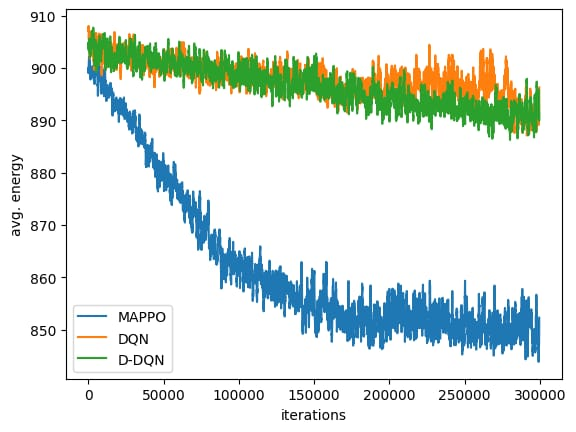
\includegraphics[width=1\columnwidth]{Energy_final.png}}
\caption{Avg. Energy vs iterations.}
\label{p3}
\end{figure}

\subsection{Comparing K-means with other clustering schemes}
In this section, we compare the performance of our K-means clustering with Hierarchical clustering and DBSCAN. Hierarchical clustering builds a hierarchy of clusters by either merging smaller clusters (agglomerative) or splitting larger ones (divisive), based on distances between points, without needing a preset number of clusters. In our comparison, we have used agglomerative hierarchical clustering. DBSCAN (Density-Based Spatial Clustering of Applications with Noise) groups points that are closely packed together based on distance and density, while marking isolated points in low-density regions as noise. Fig. {\ref{c1}} shows the variation of utility for each of the above clustering schemes. Here, K-means performs better than the other two clustering schemes. This is due to the fact that K-means works best on globular, convex, spherical clusters, which is the type of clusters we are concerned with. Moreover, according to Fig. {\ref{c2}}, K-means clustering takes significantly lesser time than the other clustering schemes. This is due to the fact K-means clustering has far less time complexity $(O(n))$ than DBSCAN $(O(nlogn))$ and Hierarchical clustering $(O(n^2))$.

\subsection{Comparing MAPPO with other policies}
We compare our work with the DRL-based Deep Q-Network (DQN) and Double Deep Q-Network (D-DQN) policies over 300,000 iterations using the same parameters to maximize utility. DQN and D-DQN are both value-based reinforcement learning algorithms that approximate Q-values using neural networks, contrasting with direct policy learning methods. As off-policy algorithms, both can learn from experiences collected using different policies than the one being optimized. Exploration is typically implemented through epsilon-greedy strategies, with random actions selected at a gradually decreasing probability to balance exploration (exploring new actions) and exploitation (choosing optimal actions). DQN achieves stability through two key innovations: experience replay buffers that break correlations in sequential data by randomly sampling stored transitions, and target networks that are periodically updated to mitigate moving target issues. D-DQN (Double DQN) extends this architecture by addressing DQN's tendency to overestimate Q-values, which can lead to suboptimal policies. It employs two separate networks—one to select actions and another to evaluate them—effectively decoupling action selection from evaluation. Both algorithms face challenges with continuous action spaces and struggle to scale efficiently to high-dimensional problems compared to policy gradient methods, explaining their lower performance in complex multi-UAV coordination tasks as shown in the comparative graphs.

We evaluated our approach by comparing its performance against DQN and D-DQN across multiple key metrics during the training process. Fig. (\ref{p1}) shows the spatial distribution of IoT devices (colored dots) grouped into clusters using K-means clustering, with each color representing a different cluster. Cluster heads are indicated by stars within each group. The red circles mark the locations of obstacles present in the environment. 

Fig. (\ref{p2}) showcases the difference between the algorithms through average utility measurements. Our algorithm(Blue Line) demonstrates remarkable improvement, beginning at negative values around -200 and climbing to consistently positive values between 400-600 by training completion, with peaks reaching 800. This represents a transformative improvement in system effectiveness. In stark contrast, both DQN and D-DQN struggle significantly, starting around -400 and barely reaching positive territory by the end of training, with maximum values only around 200. 

Similarly, Fig. (\ref{p3}) illustrates average energy consumption across the same training period, revealing our algorithm's superior energy efficiency compared to the alternatives. While all three algorithms begin with similar energy consumption levels, MAPPO demonstrates a substantial reduction by the end of training. 

Fig. (\ref{p4}) demonstrates the average Age of Information (AoI) metric. Our algorithm significantly outperforms both DQN and D-DQN by consistently achieving lower AoI values throughout the training process.A lower AoI indicates superior information freshness in the UAV network. This is critical for real-time applications where timely data is essential. 

The empirical results presented above validate the effectiveness of our approach to the utility maximization problem. Our comparative performance analysis demonstrates the algorithm's superior capability in optimizing multi-agent utility functions across diverse scenarios.
\begin{figure}
\centerline{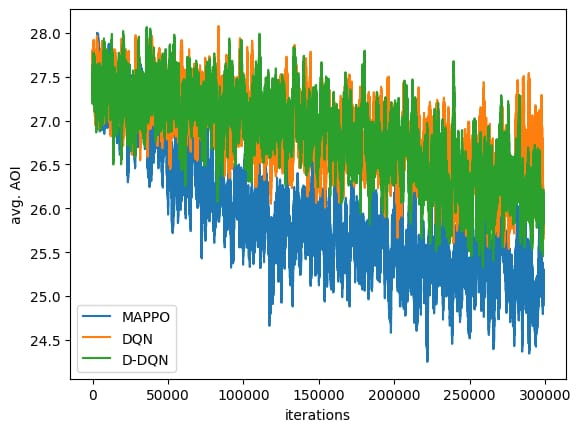
\includegraphics[width=1\columnwidth]{AOI_final.png}}
\caption{Avg. AoI vs iterations.}
\label{p4}
\end{figure}
\section{Conclusion and Future Work}
% A novel UAV-assisted data collection method for IoT networks, focusing on defense applications, has been developed. Data has been collected by the UAV from CHs in military zones. Optimization of both AoI and energy consumption has been achieved by adjusting cluster locations, UAV velocity, direction, and flying distance. Through simulations, the proposed PPO-UTP algorithm has outperformed the TD3 policy, reducing AoI and steps per episode. 
% % Future work involves exploring multi-UAV cooperative data collection in real defense environments, building on these results.

% Future work will explore multi-UAV assisted data collection method for IoT networks in real defense environments. This research will involve enhancing the current optimization techniques to accommodate multiple UAVs, ensuring efficient coordination and communication between them. Additionally, the impact of real-world factors such as varying terrain, weather conditions, and potential adversarial interference will be studied to improve the robustness and reliability of the system. The goal will be to further minimize AoI and energy consumption while maintaining high data collection efficiency in dynamic and challenging defense scenarios.

In this paper, we proposed a MAPPO-based framework for efficient task offloading and path planning in UAV-assisted IoT networks, specifically tailored for mission-critical scenarios such as defense operations. By jointly considering energy efficiency and the Age of Information (AoI), our model demonstrated significant improvements in both data freshness and energy conservation. The integration of K-means clustering and deep reinforcement learning enabled UAVs to effectively collect and relay data from IoTDs through designated cluster heads, ensuring reliable communication even in challenging terrains.

While our approach yields promising results, there are several avenues for future enhancement. Currently, both UAV-to-cluster allocation and UAV path planning are addressed under the same MAPPO framework. To improve computational efficiency and scalability, a promising direction would be to decouple UAV-to-cluster allocation as a separate subproblem. This would allow for more dynamic reassignment mechanisms in scenarios where a UAV fails or underperforms—ensuring continuous data collection by reassigning its cluster to another available UAV.

Moreover, our model assumes that UAVs operate at a fixed altitude throughout the mission. In practical deployments, allowing UAVs to adjust their altitude dynamically in response to obstacles, energy constraints, or communication quality could further optimize performance. Future work will explore the incorporation of variable-height UAV trajectory planning to enhance adaptability and mission robustness in complex environments.

\bibliographystyle{IEEEtran}
\bibliography{IEEEabrv,bibl}
\end{document}